\title{Lecture 6: Trigonometry}
\frame{\titlepage}

\begin{frame}
\frametitle{Tonight, In Your Dream}
 \begin{figure}[h!]
\centering

\includegraphics[width = 0.7\textwidth]{l09meme1}
\end{figure}
\end{frame}


\begin{frame}
\frametitle{Plotting the Sine Function}
\addfig{1}{trig_sine_circle}{\href{https://www.desmos.com/calculator/xg3bqlde8l}{Play around with this first}}{}
\end{frame}


%%%%%%%%%%%%%
\section{Triangle}
\frame{\sectionpage}
%%%%%%%%%%%%%

\begin{frame}
\frametitle{This Kind of Trinagles}
\begin{figure}[h!]
\centering

\includegraphics[width = 0.6\textwidth]{l03i02}
\end{figure}
\end{frame}

\begin{frame}
\frametitle{Vocabulary}
\begin{figure}[h!]
\centering

\includegraphics[width = 0.8\textwidth]{l09i01}
\end{figure}
\end{frame}

\begin{frame}
\frametitle{Similar Triangle}
\begin{figure}[h!]
\centering

\includegraphics[width = 0.8\textwidth]{l09i02}
\end{figure}
\end{frame}

\begin{frame}
\frametitle{Pythagorus Theorem}
\begin{figure}[h!]
\centering

\includegraphics[width = 0.6\textwidth]{l09i03}
\end{figure}
\[ a^2 + b^2 = c^2\]
\end{frame}

%%%%%%%%%%%%%
\section{Trigonometry}
\frame{\sectionpage}
%%%%%%%%%%%%%


\begin{frame}
\frametitle{Still In Your Dream}
 \begin{figure}[h!]
\centering

\includegraphics[width = 0.4\textwidth]{l09meme2}
\end{figure}
\end{frame}

\begin{frame}
\frametitle{Problem 1: Estimate the Height}
 \begin{figure}[h!]
\centering

\includegraphics[width = 0.8\textwidth]{l09i04}
\end{figure}
\end{frame}

\begin{frame}
\frametitle{Problem 2: Force}
\begin{figure}[h!]
\centering

\includegraphics[width = 0.5\textwidth]{l09i05}
\end{figure}
\end{frame}

\begin{frame}
\frametitle{Problem 3: 2D and 3D Rotation}
\begin{figure}[h!]
\centering

\includegraphics[width = 0.5\textwidth]{l09i06}
\end{figure}
\[(x,y) \then (x\cos \theta - y\sin\theta, x \sin\theta + y\cos\theta)\]
\end{frame}

\begin{frame}
\frametitle{Constants}
\begin{figure}[h!]
\centering

\includegraphics[width = 0.5\textwidth]{l09i02}
\end{figure} \pa
\[ \frac{AB}{DE} = \frac{AC}{DF} = s_1\] \pa 
\[ \frac{AB}{BC} = \frac{DE}{EF} = s_2\] \pa
\[ \frac{AC}{BC} = \frac{DF}{EF} = s_3\]
\end{frame}

\begin{frame}
\frametitle{Definition}
\begin{figure}[h!]
\centering

\includegraphics[width = 0.9\textwidth]{l09i07}
\end{figure}
\end{frame}


\begin{frame}
\frametitle{Tan(gerine)}
 \begin{figure}[h!]
\centering

\includegraphics[width = 0.7\textwidth]{l09meme3}
\end{figure}
\end{frame}

\begin{frame}
\frametitle{Definition}
\begin{figure}[h!]
\centering

\includegraphics[width = 0.6\textwidth]{l09shorthand}
\end{figure}
\end{frame}

\begin{frame}
\frametitle{Definition}
\begin{figure}[h!]
\centering

\includegraphics[width = 0.8\textwidth]{l09i08}
\end{figure}
\end{frame}


\begin{frame}[t]
\begin{ex}
Let $\theta$ be the angel indicated in the figure below. Find $\sin\theta, \cos\theta$ and $\tan\theta$.
\end{ex}
\begin{columns}
\begin{column}{0.5\textwidth}
\begin{figure}[h!]
\centering
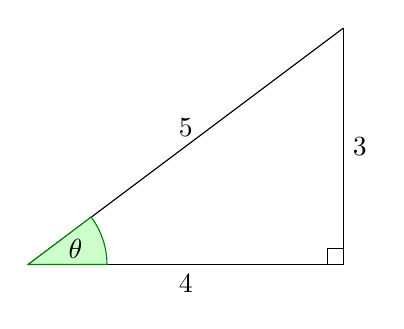
\begin{tikzpicture}
\draw (0,0) -- (4,0) node[pos=0.5, below] {4};
\draw (4,0) -- (4,3) node[pos=0.5, right] {3};
\draw (4,3) -- (0,0) node[pos=0.5, above] {5};
 \filldraw[fill=green!20!white, draw=green!50!black] (0,0) -- (10mm,0mm)
    arc [start angle=0, end angle=37, radius=10mm] -- cycle;
\draw (3.8,0) rectangle (4,0.2);
\node[black] at (0.6,0.2) {$\theta$};
\end{tikzpicture}
\caption{A triangle for example \theexample}{}
\end{figure}
\end{column}
\begin{column}{0.5\textwidth}
\begin{sol}
\begin{eq*}
\sin \theta &=& \frac{3}{5}\\
\cos \theta &=& \frac{4}{5}\\
\tan \theta &=& \frac{3}{4}
\end{eq*}
\end{sol}
\end{column}
\end{columns}
\end{frame}


\begin{frame}[t]
\begin{ex}
Let $\theta$ be the angel indicated in the figure below. Find $\sin\theta, \cos\theta$ and $\tan\theta$.
\end{ex}
\begin{columns}
\begin{column}{0.4\textwidth}
\begin{figure}[h!]
\centering
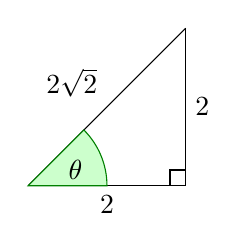
\begin{tikzpicture}
\draw (0,0) -- (2,0) node[pos=0.5, below] {2};
\draw (2,0) -- (2,2) node[pos=0.5, right] {2};
\draw (2,2) -- (0,0) node[pos=0.5, above left] {$2\sqrt{2}$};
 \filldraw[fill=green!20!white, draw=green!50!black] (0,0) -- (10mm,0mm)
    arc [start angle=0, end angle=45, radius=10mm] -- cycle;
\draw (1.8,0) rectangle (2,0.2);
\node[black] at (0.6,0.2) {$\theta$};
\end{tikzpicture}
\caption{A triangle for example \theexample}{}
\end{figure}
\end{column}
\begin{column}{0.6\textwidth}
\begin{sol}
\begin{eq*}
\sin \theta &=& \frac{2}{2\sqrt{2}} = \frac{1}{\sqrt{2}}\\
\cos \theta &=& \frac{2}{2\sqrt{2}} = \frac{1}{\sqrt{2}}\\
\tan \theta &=& \frac{2\sqrt{2}}{2\sqrt{2}} = 1 
\end{eq*}
\end{sol}
\end{column}
\end{columns}

\end{frame}


\begin{frame}[t]
\begin{ex}
Let $\Omega$ be the angel indicated in the figure below. Find $\sin\theta, \cos\theta$ and $\tan\theta$.
\end{ex}
\begin{columns}
\begin{column}{0.3\textwidth}
\begin{figure}[h!]
\centering
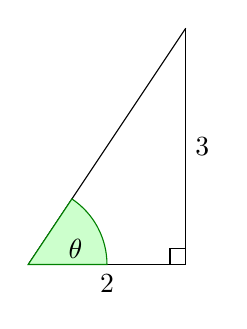
\begin{tikzpicture}
\draw (0,0) -- (2,0) node[pos=0.5, below] {2};
\draw (2,0) -- (2,3) node[pos=0.5, right] {3};
\draw (2,3) -- (0,0);
 \filldraw[fill=green!20!white, draw=green!50!black] (0,0) -- (10mm,0mm)
    arc [start angle=0, end angle=56.3, radius=10mm] -- cycle;
\draw (1.8,0) rectangle (2,0.2);
\node[black] at (0.6,0.2) {$\theta$};
\end{tikzpicture}
\caption{A triangle for example \theexample}{}
\end{figure}
\end{column}
\begin{column}{0.7\textwidth}
\begin{sol}
First we need to find the hypotenuse.
\begin{eqnarray*}
c^2 &=& a^2 + b^2 \\
c &=& \sqrt{a^2 + b^2} = \sqrt{2^2 + 3^2} = \sqrt{13}
\end{eqnarray*}
Thus
\begin{eq*}
\sin \theta &=& \frac{2}{\sqrt{13}}\\
\cos \theta &=& \frac{3}{\sqrt{13}}\\ 
\tan \theta &=& \frac{2}{3}
\end{eq*}
\end{sol}
\end{column}
\end{columns}
\end{frame}

\begin{frame}
\begin{exercisebox}{}{}
Find $\sin \theta, \cos \theta, \tan \theta$ of the following triangles.
\begin{tasks}(2)
\task 
\begin{figure}[h!]
\centering
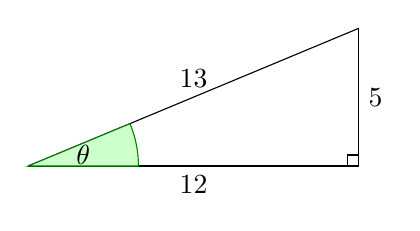
\begin{tikzpicture}[scale=0.7]
\draw (0,0) -- (6,0) node[pos=0.5, below] {12};
\draw (6,0) -- (6,2.5) node[pos=0.5, right] {5};
\draw (6,2.5) -- (0,0) node[pos=0.5, above] {13};
 \filldraw[fill=green!20!white, draw=green!50!black] (0,0) -- (20mm,0mm)
    arc [start angle=0, end angle=22.6, radius=20mm] -- cycle;
\draw (5.8,0) rectangle (6,0.2);
\node[black] at (1,0.2) {$\theta$};
\end{tikzpicture}
\end{figure}

\task 
\begin{figure}[h!]
\centering
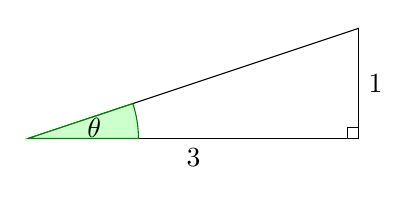
\begin{tikzpicture}[scale=0.7]
\draw (0,0) -- (6,0) node[pos=0.5, below] {3};
\draw (6,0) -- (6,2) node[pos=0.5, right] {1};
\draw (6,2) -- (0,0);
 \filldraw[fill=green!20!white, draw=green!50!black] (0,0) -- (20mm,0mm)
    arc [start angle=0, end angle=18.4, radius=20mm] -- cycle;
\draw (5.8,0) rectangle (6,0.2);
\node[black] at (1.2,0.2) {$\theta$};
\end{tikzpicture}
\end{figure}
\end{tasks}
\end{exercisebox}
\end{frame}

\begin{frame}
\frametitle{The Basic Triangles}
\begin{figure}[h!]
\centering
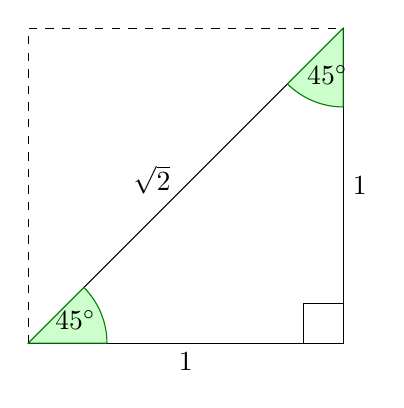
\begin{tikzpicture}
\draw (0,0) -- (4,0) node[pos=0.5, below] {1};
\draw (4,0) -- (4,4) node[pos=0.5, right] {1};
\draw (4,4) -- (0,0) node[pos=0.5, above=2pt, left=2pt] {$\sqrt{2}$};
\draw[dashed] (0,0) -- (0,4) -- (4,4);
\filldraw[fill=green!20!white, draw=green!50!black] (0,0) -- (1,0)
    arc [start angle=0, end angle=45, radius=10mm] -- cycle;
\filldraw[fill=green!20!white, draw=green!50!black] (4,4) -- (4,3)
    arc [start angle=270, end angle=225, radius=10mm] -- cycle;
\draw (3.5,0) rectangle (4,0.5);
\node[black] at (0.6,0.3) {$45^{\circ}$};
\node[black] at (3.8,3.4) {$45^{\circ}$};
\end{tikzpicture}
\caption{A right triangle with $45^{\circ}$ angles.}{}
\end{figure}
\[\sin 45^{\circ} = \cos 45^{\circ} = \frac{1}{\sqrt{2}} = \frac{\sqrt{2}}{2}\]
\end{frame}

\begin{frame}
\frametitle{The Basic Triangles}
\begin{figure}[h!]
\centering
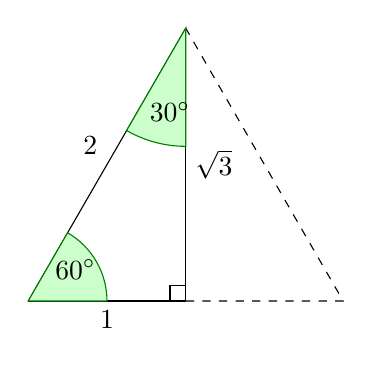
\begin{tikzpicture}
\draw (0,0) -- (2,0) node[pos=0.5, below] {1};
\draw (2,0) -- (2,3.464) node[pos=0.5, right] {$\sqrt{3}$};
\draw (2,3.464) -- (0,0) node[pos=0.5, above left] {2};
\draw[dashed] (2,0) -- (4,0) -- (2,3.464);
\filldraw[fill=green!20!white, draw=green!50!black] (0,0) -- (1,0)
    arc [start angle=0, end angle=60, radius=10mm] -- cycle;
\filldraw[fill=green!20!white, draw=green!50!black] (2,3.464) -- (2,1.964)
    arc [start angle=270, end angle=240, radius=15mm] -- cycle;
\draw (1.8,0) rectangle (2,0.2);
\node[black] at (0.6,0.4) {$60^{\circ}$};
\node[black] at (1.8,2.4) {$30^{\circ}$};
\end{tikzpicture}
\caption{A right triangle with $30^{\circ}$ and $60^{\circ}$ angle.}{}
\end{figure}
\begin{eq*}
\sin 30^{\circ} &=& \cos 60^{\circ} = \frac{1}{2} \\
\sin 60^{\circ} &=& \cos 30^{\circ} = \frac{\sqrt{3}}{2}
\end{eq*}
\end{frame}

\begin{frame}
\frametitle{Helping Hand}
\begin{table}
\centering
\begin{tabular}{|C|C|C|C|C|C|}
\hline
\theta & 0 & 30 & 45 & 60 & 90 \\
\hline
\sin & 0 & \frac{1}{2} & \frac{\sqrt{2}}{2} & \frac{\sqrt{3}}{2} & 1 \\
\hline
\cos & 1 & \frac{\sqrt{3}}{2} & \frac{\sqrt{2}}{2} & \frac{1}{2} & 0  \\
\hline
\end{tabular}
\end{table}
\addfig{0.5}{l09i10}{\href{https://www.youtube.com/watch?v=PF2nmCVSUEs&ab_channel=FuseSchool-GlobalEducation}{Hand Trick}}{}
\end{frame}

%%%%%%%%%%%%%
\section{The Unit Circle}
\frame{\sectionpage}
%%%%%%%%%%%%%

\begin{frame}
\frametitle{Revelation}
\addfig{1}{trig_plot_twist}{\href{https://www.youtube.com/watch?v=yBw67Fb31Cs&t=3508s&ab_channel=3Blue1Brown}{You have been tricked!}}{}
\end{frame}

\begin{frame}
\frametitle{}
If we fix the length of the hypotenuse to be be 1, then we reduce the functions to be
\begin{prop}{}{}
\[\sin \theta = a, \qquad \cos \theta = b, \qquad \tan \theta = \frac{a}{b} \]
\end{prop}

\begin{figure}[h!]
\centering
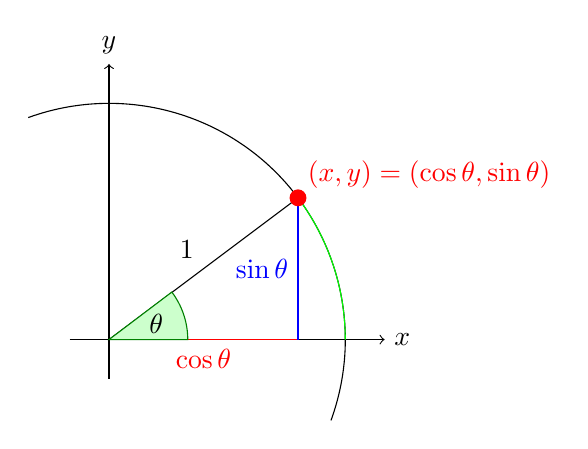
\begin{tikzpicture}
\draw[->] (-0.5,0) -- (3.5,0) node[at end, right] {$x$};
\draw[->] (0,-0.5) -- (0,3.5) node[at end, above] {$y$};
\draw (-20:3) arc  [start angle=-20, end angle=110, radius=30mm];
\draw[green] (3,0) arc  [start angle=0, end angle=37.1, radius=30mm];
\draw[red] (0,0) -- (2.4,0) node[below, pos=0.5] {$\cos \theta$};
\draw[blue] (2.4,0) -- (2.4,1.8) node[left, pos=0.5] {$\sin \theta$};
\draw (2.4,1.8) -- (0,0) node[above left, pos=0.5] {$1$};
\filldraw[fill=green!20!white, draw=green!50!black] (0,0) -- (1,0)
    arc [start angle=0, end angle=37.1, radius=10mm] -- cycle;
\node[black] at (0.6, 0.2) {$\theta$};
\filldraw[red] (2.4,1.8) circle (1mm) node[above right] {$(x,y) = (\red{\cos \theta}, \blue{\sin \theta})$};
\end{tikzpicture}
\end{figure}
\end{frame}

\begin{frame}
\frametitle{Extension}
Moreover, we can think of the hypotenuse as a radius of a circle. As we move the radius around, the angle changes.

\bigskip
Now, instead of thinking of $\sin \theta$ as the ratio between two sides, we can instead think of $\sin \theta$ as the \textbf{height} of the dot from the ground ($x$ axis). \pa 
\bigskip

Likewise, $\cos \theta$ now becomes the \textbf{distance} of the dot from the start ($y$ axis). \pa
\bigskip

This lets us extend $\theta$ to be any real number!
\end{frame}

\begin{frame}
\frametitle{Obtuse angles}
\addfig{0.6}{trig_angle_obtuse}{An obtuse angle $\theta$}{}
\end{frame}

\begin{frame}
\frametitle{Reflex angles}
\addfig{0.6}{trig_angle_reflex}{A reflex angle $\theta$}{}
\end{frame}

\begin{frame}
\frametitle{Negative angles}
\addfig{0.6}{trig_angle_minus}{A negative angle $\theta$}{}
\end{frame}

\begin{frame}
\frametitle{Summary of Signs of Trigonometry Functions}
\addfig{1}{trig_sign_summary}{A summary}{}
\end{frame}

\begin{frame}
\frametitle{Computing Sine and Cosine}
If the angle $\theta$ is between 0 and 90, you can immediately draw a triangle to find sine and cosine of that angle. 
\medskip

If not, you need to first look at the point and draw an appropriate triangle first. For instance, suppose you want to find.
\[ \sin (390) \]
First, you rotate by 390 degrees. Then, you notice that $390 = 360+30$, so the first 360 degrees rotation loops around and takes you back to the origin. Then, you rotate another 30 degrees. Hence, you have
\[ \sin (390) = \sin (360+30) = \sin (30) = \frac{1}{2}\]
We can summarize as follows.
\end{frame}

\begin{frame}[t]
\begin{prop}{}{}
\[\sin (360+\theta) = \sin \theta\]
\[\cos (360+\theta) = \cos \theta\]
\end{prop} \pa

\begin{proof}
$360 + \theta$ means going around the circle exactly once and returning to the same point, so the result stays unchanged.
\addfig{0.6}{trig_prop_360plus}{}{}
\end{proof}
\end{frame}

\begin{frame}[t]
\begin{prop}{}{}
\[\sin (180 + \theta) = - \sin \theta\]
\[\cos (180 + \theta) = - \cos \theta \]
\end{prop}

\begin{proof}
$180 + \theta$ means going around half the circle, so $\sin \theta$ changes sign (from up to down) and so does $\cos \theta$ (from left to right).
\addfig{0.5}{trig_prop_180plus}{}{}
\end{proof}
\end{frame}

\begin{frame}[t]
\begin{ex}
Find $\sin (180 - \theta)$ and $\cos (180 - \theta)$ in terms of $\sin \theta$ and $\cos \theta$.
\end{ex}

\begin{sol}
Looking at the graph, we see that $180 - \theta$ degrees is the reflection of the angle $\theta$ across the y-axis. Thus, the height is the same, so $\sin (180 - \theta) = \theta$ and and width becomes negative so $\cos(180 - \theta) = -\cos(\theta)$.
\addfig{0.5}{trig_prop_180minus}{}{}
\end{sol}
\end{frame}

\begin{frame}[t]
\begin{ex}
Find $\sin (90 - \theta)$ and $\cos (90 - \theta)$ in terms of $\sin \theta$ and $\cos \theta$.
\end{ex}
\begin{sol}
If you draw a triangle with angle $90 - \theta$ degrees, you will notice that the other angle in the triangle, labeled $\alpha$ is exactly $\theta$. This is because we know that the sum of all three angles are 180, so $90 + (90 - \theta) + \alpha = 180$, giving us $\alpha = \theta$.
\addfig{0.5}{trig_prop_90minus1}{}{}
\end{sol}
\end{frame}

\begin{frame}[t]
\begin{sol} (Continued)
Then, if we focus on the other triangle, we get the following figure.
\addfig{0.5}{trig_prop_90minus2}{}{}
Notice that the sine and cosine switch place. This is because we rotate the triangle by 90 degrees, so height becomes width and vice versa. Thus, if we compare this new triangle to the original triangle, we get

\[\sin (90 - \theta) = \cos \theta\]
\[\cos (90 - \theta) = \sin \theta \]
\end{sol}
\end{frame}

\begin{frame}
\begin{exercisebox}{}{}
Find the following expressions in terms of $\sin \theta$ and $\cos \theta$.
\begin{tasks}(1)
\task $\sin (90 + \theta)$ and $\cos (90 + \theta)$
\task $\sin (- \theta)$ and $\cos (- \theta)$
\task $\sin (270 + \theta)$ and $\cos (270 + \theta)$
\task $\tan (90 - \theta)$ and $\tan (90 + \theta)$
\end{tasks}
\end{exercisebox}
\end{frame}

%%%%%%%%%%%%%
\section{Identity}
\frame{\sectionpage}
%%%%%%%%%%%%%

\begin{frame}[t]
\frametitle{Some Identity}
\begin{block}{}
\[\sin^2 \theta + \cos^2 \theta = 1\]
\end{block}

\begin{proof}
\begin{eqnarray*}
\sin^2 \theta + \cos^2 \theta \pa &=& \left(\frac{a}{c}\right)^2 + \left(\frac{b}{c}\right)^2 \\
\pa &=& \frac{a^2}{c^2} + \frac{b^2}{c^2} \\
\pa &=& \frac{a^2 + b^2}{c^2} \\
\pa &=& \frac{c^2}{c^2}  \\
\pa &=& 1
\end{eqnarray*}
\end{proof}
\end{frame}

\begin{frame}[t]
\begin{alertblock}{}
\[\sin(\alpha + \beta) \neq \sin(\alpha) + \sin(\beta)\]
\end{alertblock}

You can see easily that this is not the case by trying some angles (say $\alpha = \beta = 30$).

Instead, we have 

\begin{block}{}
\[\sin(\alpha + \beta) = \sin\alpha\cos\beta + \sin\beta\cos\alpha\]
\end{block}

We do not need this for this introductory course, and the proof is quite complicated, so we'll leave it. Nevertheless, if you are given an identity, you should be able to use it to find some other values.
\end{frame}


\begin{frame}[t]
\begin{ex}
Given the identity $\sin^2 \alpha + \cos^2 \alpha = 1$ and that $\sin 37 \approx 0.6$, find $\cos 37$.
\end{ex}
\begin{sol}
We can simplify the identity to be
\begin{eq*}
\cos^2 \alpha &=& 1 - \sin^2\alpha \\
\cos\alpha &=& \sqrt{1-\sin^2\alpha}
\end{eq*}
Thus, if we plug it $\alpha = 37$, we get
\begin{eq*}
\cos 37 &=& \sqrt{1- \sin^2 (37)} \\
&=& \sqrt{1 - (0.6)^2} \\
&=& \sqrt{0.64} = 0.8
\end{eq*}
\end{sol}
\end{frame}


\begin{frame}[t]
\begin{ex}
Given the identity $\cos \frac{\alpha}{2} = \sqrt{\frac{1+\cos(\alpha)}{2}}$ and that $\cos 60 = \frac{1}{2}$. Find the value of $\cos 30$.
\end{ex}
\begin{sol}
If we plug in the value $\alpha = 60$, we have
\begin{eq*}
\cos \frac{60}{2} &=& \sqrt{\frac{1+\cos 60}{2}} \\
\cos 30 &=& \sqrt{\frac{1+\frac{1}{2}}{2}} \\
&=& \sqrt{\frac{3}{4}} \\
&=& \frac{\sqrt{3}}{2}
\end{eq*}
\end{sol}
\end{frame}


\begin{frame}[t]
\begin{ex}
Given the identity $\sin (2\alpha) = 2\sin\alpha \cos \alpha$ and that $\sin 30 = \frac{1}{2}$. Find the value of $\sin 60$.
\end{ex}
\begin{sol}
If we plug in the value $\alpha = 30$, we have
\[\sin 60 = 2 \sin 30 \cos 30\]
We don't know the value of $\cos 30$ yet, but of course we can use the pythagorean theorem to get
\[\cos 30 = \sqrt{1-\sin^2 (30)} = \sqrt{1 - \left(\frac{1}{2}\right)^2} = \sqrt{\frac{3}{4}} = \frac{\sqrt{3}}{2}\]
Therefore,
\[\sin 60 = 2 \sin 30 \cos 30 = 2 \left(\frac{1}{2}\right) \left(\frac{\sqrt{3}}{2}\right) =  \frac{\sqrt{3}}{2}\]
\end{sol}
\end{frame}

\begin{frame}
\frametitle{Trigoromantic}
 \begin{figure}[h!]
\centering

\includegraphics[width = 0.4\textwidth]{l09meme4}
\end{figure}
\end{frame}

\begin{frame}
\frametitle{But There Is More!}
 \begin{figure}[h!]
\centering

\includegraphics[width = 0.7\textwidth]{l09meme5}
\end{figure}
\end{frame}

\begin{frame}
\begin{exercisebox}{}{}
\begin{tasks}(1)
\task Given that $\sin \beta = \frac{1}{4}$ for some angle $\beta$, find $\cos \beta$.
\task Given the identity $\cos (2\alpha) = 1-2\sin^2 (\alpha)$ and the value $\sin (45) = \frac{\sqrt{2}}{2}$, find $\cos 90$.
\task Use the identity $\cos (2\alpha) = 2\cos^2 (\alpha)-1$ to find the solutions of $\cos (2\alpha) = \cos\alpha$ for $0 \leq \alpha \leq 360$. Also plot the graph of $f(x) = \cos(2\alpha)$ and $g(x) = \cos\alpha$ to verify that you get all the solutions.
\end{tasks}
\end{exercisebox}
\end{frame}


%%%%%%%%%%%%%
\section{Trigonometry Function}
\frame{\sectionpage}
%%%%%%%%%%%%%

\begin{frame}
\frametitle{There is a Numberphile Clip for That!}
\addfig{0.9}{numberphile_trig}{\href{https://www.youtube.com/watch?v=snHKEpCv0Hk}{Beautiful Trigonometry - Numberphile}}{}
\end{frame}


\begin{frame}
\frametitle{Trigonometry as Functions}
Since trigonometry functions are, evidently, functions, we can plot them!
\begin{defn}{}{}
For any real number $x$, define the function
\[f(x) = \sin x\]
where the domain is the set of all real numbers $\mathbb{R}$ and the range is the interval $[-1,1]$. Similarly, define
\[f(x) = \cos x\]
\end{defn}
\end{frame}

\begin{frame}
\begin{figure}[h!]
\centering

\includegraphics[width = 0.6\textwidth]{l09i12}
\end{figure}
These functions are commonly used to model physical behaviors such as
\begin{itemize}
\item Wave \pa
\item Oscillation \pa 
\item Periodic \pa
\end{itemize}
\end{frame}

%%%%%%%%%%%%%
\section{Extra}
\frame{\sectionpage}
%%%%%%%%%%%%%

\begin{frame}
\frametitle{The Whole Family}
Note: We also define the following functions
\[ \sec \theta = \frac{1}{\sin \theta}\pa, \quad \csc \theta = \frac{1}{\cos \theta}\pa, \quad\cot \theta = \frac{1}{\tan \theta}\] \pa

These notations are handy when dealing with some types of problems, but we do not need them for now.
\end{frame}

\begin{frame}
\frametitle{Sine, Sine Everywhere}
\addfig{0.9}{wait_its_all_sine}{Mind=Blown}{}
\end{frame}

\begin{frame}
\frametitle{$\pi$}
In mathematics, we use a different unit of angle, called \textbf{radian}. Instead of defining $\sin$ to be the ratio between sides of the triangle, we define it to be the length of the arc of the unit circle.

\begin{block}{}
\[ \pi = 180^{\circ}\]
\end{block}

For instance, 
\begin{eqnarray*}
\cos \pi &=& \cos 180^{\circ} = -1 \\
\sin 2\pi &=& \sin 360^{\circ} = 0\\
\sin \frac{\pi}{2} &=& \sin 90^{\circ} = 1
\end{eqnarray*}
\end{frame}

\begin{frame}
\frametitle{Inverse Trigonometry Functions}
There are associated inverse functions, namely
\[ \arcsin A, \arccos A, \arctan A\]
If $\sin \theta = A$, then we simply have $\arcsin A = \theta$. Since $\sin \theta$ expresses the ratio between two sides of the triangles, $\arcsin A$ expresses the angle such that such ratio is $A$.

\begin{exampleblock}{Example}
\begin{itemize}
\item We know that $\sin 30^{\circ} = \frac{1}{2}$, so we have $\arcsin \frac{1}{2} = 30^{\circ}$
\item We know that $\cos 60^{\circ} = \frac{1}{2}$, so we have $\arccos \frac{1}{2} = 60^{\circ}$
\item We know that $\tan 45^{\circ} = 1$, so we have $\arctan 1 = 45^{\circ}$
\end{itemize}
\end{exampleblock}
\end{frame}

\begin{frame}
\frametitle{Fun Fact}
Then, you may wonder why we used 360 in the first place? The number itself seems arbitrary.
\bigskip

Answer: Because it has lots of divisors, namely
\[1,2,3,4,5,6,8,10,12,15,18,20,24, 30, 36, 40, 60, 72, 90, 120, 180, 360\]
\end{frame}

\begin{frame}
\frametitle{Extending the Unit Circle}
There are geometrical explanations for other trigonometric functions.
\begin{figure}[h!]
\centering
\begin{tikzpicture}
\draw[<->] (-3.5,0) -- (4,0) node[at end, right] {$x$};
\draw[<->] (0,-0.5) -- (0,5.5) node[at end, above] {$y$};
\draw (3,0) arc [start angle = 0, end angle = 180, radius = 30mm];
\draw[red, dashed] (0,0) -- (2.4,0);
\draw[green] (2.4,0) -- (2.4,1.8) node[left, pos=0.5] {$\sin \theta$};
\draw (2.4,1.8) -- (0,0) node[above left, pos=0.5] {$1$};
\filldraw[fill=green!20!white, draw=green!50!black] (0,0) -- (1,0)
    arc [start angle=0, end angle=37.1, radius=10mm] -- cycle;
\node[black] at (0.6, 0.2) {$\theta$};
\draw (2.2,0) rectangle (2.4,0.2);
\draw[red] (0,1.8) -- (2.4,1.8) node[above, pos=0.5] {$\cos \theta$};
\draw[magenta] (0,0) -- (3.75,0) node[below, pos=0.5] {$\text{sec } \theta$};
\draw[cyan] (0,0) -- (0,5) node[left, pos=0.5] {$\text{csc } \theta$};
\draw[purple] (0,5) -- (2.4,1.8) node[above, right, pos=0.5] {$\text{cot } \theta$};
\draw[orange] (2.4,1.8) -- (3.75,0) node[above, right, pos=0.5] {$\tan \theta$};
\draw[rotate = 217.1, xshift=24mm, yshift=18mm] (0,0) rectangle (0.2, 0.2);
\end{tikzpicture}
\caption{Geometrical interpretations of all six trigonometry functions.}
\end{figure}
\end{frame}



